\documentclass[12pt,fullpage, a4paper]{article}
\usepackage[
margin=1.5cm,
includefoot,
footskip=30pt,
]{geometry}
%\usepackage[utf8x]{inputenc}
%\usepackage[T1]{fontenc}
\usepackage{amsmath}
\usepackage{amsfonts}
\usepackage{amssymb}
\usepackage{graphicx}
\usepackage{comment}
\usepackage[authoryear, comma]{natbib}
\usepackage{lineno}
\usepackage{url}



\linenumbers
%\bibliographystyle{evolution.bst}
%\bibliographystyle{plainnat}

\newcommand{\norm}[1]{\left\lVert#1\right\rVert}
\newcommand{\normsq}[1]{\left\lVert#1\right\rVert^2}
\newcommand{\MX}{\mathbf{X}} %uncentered data
\newcommand{\MC}{\mathbf{C}} %centering
\newcommand{\MY}{\mathbf{Y}} %centered data
\newcommand{\MF}{\mathbf{F}_2} %F2-distance matrix
\newcommand{\MFT}{\mathbf{F}_3} %F3-distance matrix
\newcommand{\MP}{\mathbf{P}} % PCs
\newcommand{\ML}{\mathbf{L}} % loadings
\newcommand{\MK}{\mathbf{K}} % Kernel
\newcommand{\MSINGULAR}{\mathbf{\Sigma}} % Singular values matrix
\newcommand{\MEIGEN}{\mathbf{\Lambda}} % Eigenvalue matrix
\newcommand{\MEAN}{\boldsymbol{\mu}} % Kernel
\title{Modelling complex population structure using $F$-statistics and Principal Component Analysis}
\author{Benjamin M Peter}
\begin{document}
	\maketitle
\begin{abstract}
Human  genetic diversity is shaped by our complex history. Population genetic tools to understand this variation can broadly be classified into data-driven methods such as Principal Component Analysis (PCA), and model-based approaches such as $F$-statistics.
Here, I show that these two perspectives are closely related, and I derive explicit connections between the two approaches. I show that $F$-statistics have a simple geometrical interpretation in the context of PCA, and that orthogonal projections are the key concept to establish this link. I illustrate my results on two examples, one of local, and one of global human diversity. In both examples, I find that population structure is sparse, and only a few components contribute to most statistics. Based on these results, I develop novel visualizations that allow for investigating specific hypotheses, checking the assumptions of more sophisticated models. My results extend $F$-statistics to non-discrete populations, moving towards more complete and less biased descriptions of human genetic variation.
\end{abstract}
\section{Introduction}
Most genetic variation in humans is shared between all of us, but around 15\% of genetic variation in humans can be explained by population structure \citep{dobzhansky1972, barbujani1997, rosenberg2002a}. Genome-scale data has allowed us to leverage the information contained in these 15\% to study our genetic diversity and history in great detail \citep{cavalli-sforza1994,reich2018a}. For some data sets it is possible to predict an individuals origin at a resolution of a few hundred kilometers \citep{novembre2008, leslie2015}, and direct-to-consumer-genetics companies are using this variation to analyze the genetic data of millions of customers.

However, understanding, conceptualizing and modeling this variation is far from trivial, particularly since misconstrued models of human genetic differentiation have repeatedly been used to justify racist, eugenic and genocidal policies. Lewontin's landmark \citeyear{dobzhansky1972} paper on the apportionment of human genetic diversity was one of the first to question ``races'' not only on ethical, but also on scientific grounds. In Lewontin's data, less than half of the already small proportion of between-population genetic variation can be attributed to ``racial'' continental-scale groupings. Over the last five decades, this view has been corroborated and extended many times \citep{cann1987, cavalli-sforza1994, cann2002, rosenberg2002, reich2018a}, and we now know that human races are an arbitrary, biologically useless polyphyletic grouping that is maintained by historical and social conventions.

Modern descriptions of human genetic diversity focus on the evolutionary processes that caused it, and which gives rise to  both discrete and continuous components \citep{rosenberg2002a, serre2004, rosenberg2005, bradburd2018, reich2018a}. In isolation, populations are expected to slowly diverge, particularly if they are separated by barriers to migration such as mountain ranges, oceans or deserts \citep{bradburd2013, peter2020a, rosenberg2005}. On the other hand, major population movements such as the out-of-Africa, Austronesian or Bantu expansions lead to more gradual patterns of genetic diversity \citep{cavalli-sforza1994, ramachandran2005, novembre2008, peter2020a, stoneking2016, racimo2020}. Local migration between neighboring populations will flatten differentiation, and long-distance migrations \citep{alves2016} or secondary contact and admixture between diverged populations, such as Neandertals and modern humans \citep{green2010},will lead to locally increased diversity.

This complex population structure is frequently handled by using multiple models with different assumptions; each emphasizing a particular aspects of the data. Data-driven methods such as Principal Component Analysis (PCA, \cite{cavalli-sforza1994}) structure \citep{pritchard2000} or multidimensional scaling (MDS, \cite{malaspinas2014}) are often used to display the full complexity of the data, but they have the disadvantage that they are not easily interpretable. For this purpose, more explicit demographic models \citep{gutenkunst2009, kamm2015, excoffier2013} are applied, which allow for parameter estimation or hypothesis tests. 

Particularly in the analysis of human ancient DNA, a set of techniques based on $F$-statistics \textit{sensu} Patterson have risen in popularity \citep{patterson2012, peter2016}. This framework is based on the null-assumption that the relationship between  populations is tree-like, and then uses tests involving three or four populations to probe for violations of treeness \citep{patterson2012}. In a further step, $F$-statistics of multiple populations can be combined to estimate parameters in more complex models \citep{patterson2012, harney2021}. However, the connections between PCA, $F$-statistics and explicit demographic models are often unclear, which makes quantitative comparisons, detecting model violations and joint interpretation of these approaches difficult. Since both $F$-statistics and PCA are functions of expected pairwise coalescent times \citep{mcvean2009, peter2016}, this is one avenue to link these approaches. Here, I instead use the geometric interpretation of $F$-statistics developed by  \cite{oteo-garcia2021} to directly visualize $F$-statistics on a PCA plot. 

	
\section{Theory}
In this section, I will give a very brief formal introduction to $F$-statistics and PCA. A more detailed technical treatise of PCA is given by e.g. \cite{jolliffe2013} and \cite{pachter2014}, and a useful guide to interpretation is \cite{cavalli-sforza1994}. Readers unfamiliar with $F$-statistics may find \cite{patterson2012}, \cite{peter2016} or \cite{oteo-garcia2021} helpful.

\subsection{Introduction to PCA}
Let us assume we have some genotype data summarized in a matrix $\MX$ whose entry $x_{ij}$ reflects the allele frequency of the $i$-th population at the $j$-th genotype. If we have $S$ SNPs and $n$ populations, $\MX$ will have dimension $n \times S$. As a population may be represented by just one individual, there is no conceptual difference between an individual-based and population-based analysis. Since the allele
frequencies are between zero and one, we can interpret each Population $X_i$
of $\MX$ as a point in $[0, 1]^S$, the allele frequency or \emph{data space}.
	
The goal of PCA is to find a low-dimensional subspace $\mathbb{R}^K$ that explains most of the variation in the data. $K$ is at most $n-1$, in which case the data is simply rotated. However, the  historical processes that generated genetic variation often result in \emph{sparse} data \citep{engelhardt2010}, so that $K \ll n$ explains a substantial portion of the variation; for visualization $K=2$ is frequently used. 
	
	
There are several algorithms that are used to perform PCAs, the most common one is based on singular value decomposition \citep{jolliffe2013}. In this approach, we first mean-center $\MX$, obtaining a centered matrix $\MY$
	\begin{equation*}
	y_{il} = x_{il} - \mu_l
	\end{equation*}
	where $\mu_l$ is the mean allele frequency at the $l$-th locus.
	
	PCA can then be written as
	
	\begin{equation}
	\MY = \MC\MX = (\mathbf{U} \MSINGULAR) \mathbf{V}^T = \MP\ML\text{,}
	\end{equation}
	
	where $\MC = \mathbf{I} -\frac{1}{n}\mathbf{1}$ is a centering matrix that subtracts row means, with $\mathbf{I}, \mathbf{1}$  the identity matrix and a matrix of ones, respectively. The orthogonal matrix of principal components $\MP=\mathbf{U}\MSINGULAR$ has size $n \times n$ and is used to reveal population structure. The SNP loadings $\ML=\mathbf{V}^T$ are an orthonormal matrix of size $n \times S$, its rows give the contribution of each SNP to each PC, it is often useful to look for outliers that might be indicative of selection \citep[e.g][]{francois2010}.
	
	In many  implementations \citep[e.g.][]{patterson2006}, SNPs are weighted by
    the inverse of their standard deviation. As this weighting often makes little
    difference in practice \citep{mcvean2009}, I will assume throughout that SNPs
    are unweighted.

\subsection{Introduction to $F$-statistics}
PCA is typically used to model population structure between many populations. $F$-statistics take the opposite approach, revealing the relationship between just two,  three or four populations at a time. The three $F$-statistics can be defined as 
\begin{subequations}
	\begin{align}
	&F_2(X_1, X_2) &=& \frac{1}{S}\sum_{l=1}^S(x_{1l} - x_{2l})^2
	&=& \frac{1}{S}\langle X_1 - X_2, X_1 - X_2 \rangle = \frac{1}{S}\normsq{X_1-  X_2}\\
	&F_3(X_1; X_2, X_3) &=& \frac{1}{S}\sum_{l=1}^S(x_{1l} - x_{2l})(x_{1l} - x_{3l}) &=& \frac{1}{S}\langle X_1 - X_2, X_1 - X_3 \rangle\\	
	&F_4(X_1, X_2; X_3, X_4) &=& \frac{1}{S}\sum_{l=1}^S(x_{1l} - x_{2l})(x_{3l} - x_{4l}) &=& \frac{1}{S}\langle X_1 - X_2, X_3 - X_4 \rangle	\text{,}
	\end{align}
\end{subequations}
where $\norm{\cdot}$ denotes the Euclidean norm and $\langle \cdot, \cdot \rangle$ denotes the dot product. The normalization by the number of SNPs $S$ is assumed to be the same for all calculations and is thus omitted subsequently. Some elementary properties of the dot product between vectors $a, b, c$ that I will use later are
\begin{subequations}
\begin{align}
\langle a, b \rangle &= \sum_i a_ib_i\\
\langle a, b \rangle &= \norm{a}\norm{b}\cos(\phi)\\
\langle a, a \rangle &= \normsq{a}\\
\langle a + c, b \rangle &= \langle a, b \rangle + \langle b, c \rangle,
\end{align}
\end{subequations}
where $\phi$ is the angle between $a$ and $b$. 

 Furthermore, both $F_3$ and $F_4$ can be written as sums of $F_2$-statistics:
\begin{subequations}
	\begin{align}
2F_3(X_1; X_2, X_3) &= F_2(X_2, X_3) - F_2(X_1, X_2) - F_2(X_1, X_3)\label{eq:f3fromf2}\\
2F_4(X_1, X_2; X_3, X_4) &= F_2(X_1, X_3) + F_2(X_2, X_4) - F_2(X_1,X_4) - F_2(X_2, X_3)\label{eq:f4fromf2}
	\end{align}
\end{subequations}

$F$-statistics have been primarily motivated in the context of trees and admixture graphs \citep{patterson2012}. In a tree, the squared Euclidean distance $F_2(X_1, X_2)$ measures the length of all branches between populations $X_1$ and $X_2$; and $F_3$ and $F_4$ represent external and internal branches in a tree, respectively \citep{peter2016}. The length is a measure of genetic drift, and is non-negative if data is generated under a tree \citep{patterson2012}. This interpretation is useful to understand a number of applications. The outgroup-$F_3$-statistic $F_3(O; U, X_i)$, for example, is useful if we have an unknown population $U$, and want to find its closest relatives from a panel of populations $X_i$. The highest values of $F_3$ indicate the population $X_i$ most closely related to $U$, using the outgroup $O$ to correct for differences in sample times. The population $X_i$ with the largest value is the most closely related population out of the reference sample. The internal branches described by  $F_4$-statistics are frequently used for complex models, such as  reconstructing admixture graphs \citep{patterson2012, lipson2013} and estimating admixture proportions \citep{petr2019, harney2021}.

Most commonly however, $F_3$ and $F_4$ are used as admixture tests \citep{patterson2012}: Negative values of  $F_3(X_1; X_2, X_3) < 0$ correspond to a branch with negative genetic drift, which is a violation of treeness. Similarly if four populations are related as a tree, then at least one of the $F_4$ statistics between the populations will be zero \citep{patterson2012}.

To move away from trees and graph models, I build upon the geometric framework of \cite{oteo-garcia2021}. Here, we think of each population as a point in the data space $\mathbb{R}^S$, made up of the allele frequency at each SNP. Then, $F_2(X_1, X_2) = \normsq{X_1 - X_2}$ is the squared Euclidean distance between two populations $X_1$ and $X_2$, and $F_4(X_1, X_2 ; X_3, X_4) = \langle X_1 - X_2, X_3 - X_4 \rangle$ is the inner (dot) product between these two vectors. These dot products are useful for a variety of projections that use population structure.

\subsection{Connection between PCA and $F$-statsitics}	
\subsubsection{Principal components from $F$-statistics}
PCA and $F$-statistics are closely related. In fact, the principal components can be directly calculated from $F$-statistics using multidimensional scaling, which, for squared Euclidean ($F_2$)-distances, leads to an identical decomposition to PCA \citep{gower1966}. Suppose we calculate the pairwise $F_2(X_i, X_j)$ between all $n$ populations, and collect them in a matrix $\MF$. We can obtain the principal components from this matrix by double-centering it, so that its row and column means are zero, and perform an eigendecomposition of the resulting matrix:
\begin{equation}
\MP\MP^T = - \frac{1}{2}\MC\MF\MC \text{.} \label{eq:mds}
\end{equation}

\subsubsection{$F$-statistics in PCA-space}
By performing a PCA, we rotate our data to reveal the axes of highest variation. However, the dot product is invariant under rotation, and $F$-statistics can be thought of as dot products.  What this means is that we are free to calculate $F_2$ either on the uncentered data $\MX$, the centered data $\MY$ or any other orthogonal basis such as the principal components $\MP$. Formally,

\begin{align}
F_2(X_i, X_j) &=&  \sum_{l=1}^L \big( x_{il} -x_{jl}\big)^2  &&\nonumber\\ 
&=& \sum_{l=1}^L \big( (x_{il} - \mu_l) -(x_{jl} -\mu_l)\big)^2   &=& F_2(Y_i, Y_j) \nonumber\\
&=& \sum_{k=1}^n (p_{ik} - p_{jk})^2  &=& F_2(P_i, P_j) \text{,}\label{eq:fpc}
\end{align}
A derivation of this change-of-basis is given in Appendix \ref{appendix:fonpc}, Equation \ref{eq:changeofbasis}.
As $F_3$ and $F_4$ can be written as sums of $F_2$-terms (Eqs. \ref{eq:f3fromf2}, \ref{eq:f4fromf2}), analogous relations apply.

In most applications, we do not use all PCs, but instead truncate to the first $K$ PCs, which explain most of the between-population genetic variation.
Thus, 
\begin{equation}
F_2(P_i, P_j) = \underbrace{\sum_{k=1}^K(p_{ik} - p_{jk})^2}_{\hat{F_2}^{(K)}(P_i, P_j)} + \sum_{k=K+1}^n(p_{ik} - p_{jk})^2 \text{.}
\end{equation}
If we sum up the approximation errors $F_2 - \hat F_2$ over all pairs of populations, we obtain the Frobenius-norm of the error $\normsq{\MF - \hat{\MF}}_F$; which is precisely the function that is minimized in MDS \citep{jolliffe2013}. Thus, $\hat\MF^{(K)}$ is an optimal sparse approximation of $\MF$ for any $K$.

\section{Material \& Methods}
The theory outlined in the previous section suggests that $F$-statistics have a geometric interpretation in PCA-space, which can be approximated on PCA plots. In the next section I explore this connection in detail, and illustrate it on two sample data sets that I briefly introduce here. Both are based on the analyses by \cite{lazaridis2014}. The data is from the Reich lab compendium data set (v44.3), downloaded from \url{https://reich.hms.harvard.edu/allen-ancient-dna-resource-aadr-downloadable-genotypes-present-day-and-ancient-dna-data}, using data on the ``Human Origins''-SNP set (597,573 SNPs). SNPs with missing data in any population are excluded. The code used to create all figures and analyses will be available on \url{https://github.com/BenjaminPeter/fstats_pca}.

\paragraph{``World'' data set}
This data set represents global human genetic variation (638 individuals from 33 population), as used by \citep{lazaridis2014}. As this data set is very sparse, it may be well-approximated by an admixture graph.


\paragraph{West-Eurasian data set}
This data set of 1,119 individuals from 62 populations contains  present-day individuals from the Eastern Mediterranean, Caucasus and Europe. It is frequently used as a basis of comparison for ancient genetic analyses of Western Eurasian individuals \citep{patterson2012, lazaridis2014}. Genetic differentiation in this region is low and closely mirrors geography \citep{novembre2008}, and thus may not be particularly graph-like.


\paragraph{Computing $F$-statistics and PCA}
I perform analyses at the level of populations to ease presentation.  It is an assumption of $F$-statistics that the genetic variation within sampled population is independent of the variation between samples \citep{patterson2012}. All computations are performed in \texttt{R}. I use \texttt{admixtools 2.0.0} (\url{https://github.com/uqrmaie1/admixtools}) to compute $F$-statistics. To obtain a PC-decomposition, I first calculate all pairwise $F_2$-statistics, obtain a nearby negative semidefinite matrix using the \texttt{nearPD} function, and then use equation \ref{eq:mds} and the \texttt{eigen} function to obtain the PCs. 

\section{Results}

\begin{figure}[!ht]
	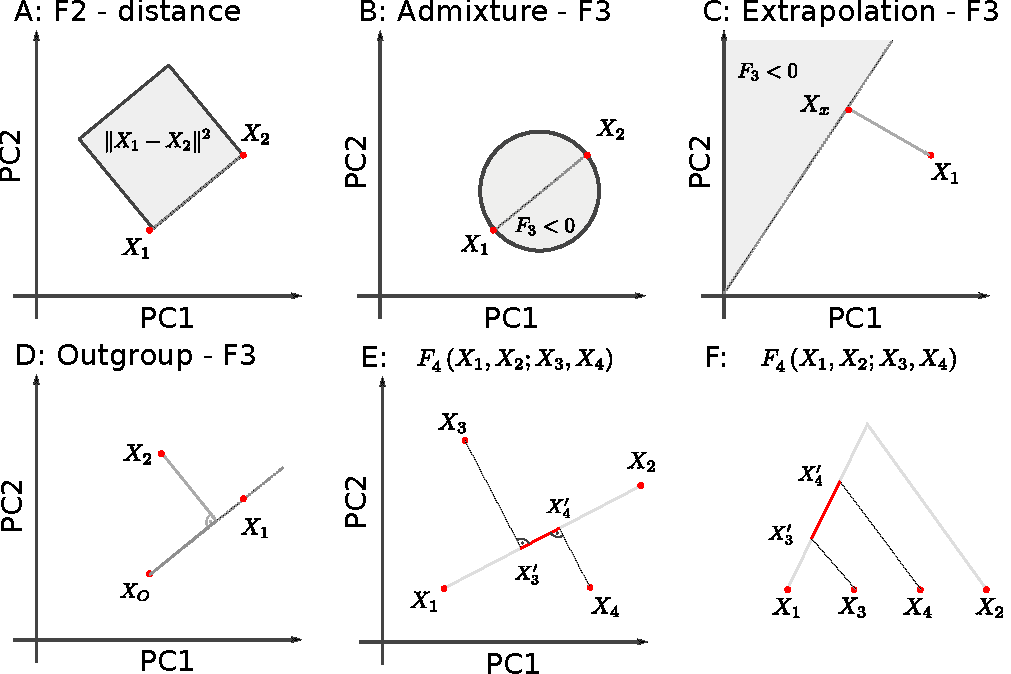
\includegraphics[width=\textwidth]{figures/fstats_on_pca.pdf}
	\caption{\textbf{Geometric representation of $F$-statistics on 2D-PCA-plot.} A: $F_2$ represents the squared Euclidean distance between two points in PC-space. B: Admixture-$F_3(X_x; X_1, X_2)$ is negative if $X_x$ lies in the circle specified by the diameter $X_2-X_1$. C: $F_3(X_x; X_1, X_2)$ is negative given $X_1, X_x$ if $X_2$ is in the gray space.  D: Outgroup-$F_3$ reflects the projection of $X_2 - X_O$ on $X_1 - X_O$. E: $F_4$ is the projection of $X_3 - X_4$ on $X_1-X_2$. F: Same projection, but assuming data is generated by a tree.}
	\label{fig:geom}
\end{figure}

%\subsection{Geometry of $F$-statistics in PC-space}
The transformation from the previous section allows us to consider the geometry
of $F$-statistics in PCA-space. The relationships we will discuss formally only
hold if we use all $n-1$ PCs. However, the appeal of PCA is that frequently,
only a very small number $K \ll n$ of PCS contain most information that is
relevant for population structure (for visualization
$K=2$ is often used).

\subsection{$F_2$ in PC-space}
The $F_2$-statistic is an estimate of the squared Euclidean distance between two
populations. It thus corresponds to the squared distance between populations in PCA-space, and
reflects the intuition that closely related populations  will be close to each other on a
PCA-plot, and have low pairwise $F_2$-statistics. In converse, if two
populations have high $F_2$ but appear on the same point on an PCA-plot, this suggests
that substantial variation is hidden on higher PCs.


\subsection{When are admixture-$F_3$ statistics negative?}
Given two source populations $X_1$, $X_2$, can we predict which populations $X_x$ could be considered admixed between these populations based on PCA? Since the allele frequencies of $X_x$ are intermediate between those of $X_1$ and $X_2$, we would expect it to lie between $X_1$ and $X_2$, with the exact location depending on sample sizes \citep{brisbin2012, mcvean2009}. 

The $F_3$-statistic gives a more precise interpretation: we are looking for the space where $F_3$ is negative, i.e. 
\begin{eqnarray}
2 F_3(X_x; X_1, X_2) &=& 2\langle  X_x - X_1, X_x - X_2 \rangle \nonumber\\
      &=& \normsq{X_x - X_1} + \normsq{X_x - X_2}  - \normsq{X_1 - X_2} < 0 \label{eq:f3neg}
\end{eqnarray}
By the Pythagorean theorem, $F_3 = 0 $ if and only if $X_1, X_2$ and $X_x$ form a right-angled triangle. The associated region where $F_3=0$ is a $n$-sphere (or a circle in two dimensions) with diameter $\overline{X_1X_2}$. $F_3$ is negative when the triangle is obtuse, i.e. $X_x$ is admixed if it lies inside the $n$-ball with diameter $\overline{X_1X_2}$ (Figure \ref{fig:geom}B, Equation \ref{eq:f3sphere}). 

\paragraph{$F_3$ on a 2D-plot.} 
 If we project this $n$-ball on a two-dimensional plot, $\overline{X_1X_2}$ will usually not align with the PCs; thus the ball may be somewhat larger. This geometry is perhaps easiest visualized on a globe. If we look at the globe from a view point parallel to the equator, both the north and south poles are visible at the very edge of the circle. But if we look at it from above the north pole, the north- and south-poles will be at the very same point.
 
 Thus if $\hat{F}_3 \ll F_3$, the true circle will be bigger than would be predicted from a 2D-plot. In this case, substantial relevant genetic differentiation is ``hidden'' in the higher PCs, and populations that appear inside the circle on a PCA-plot may, in fact, have positive $F_3$-statistics. This is because they are outside the $n$-ball in higher dimensions. The converse interpretation is more strict: if a population lies outside the circle on \emph{any} 2D-projection, $F_3$ is guaranteed to be bigger than 0 (see Equation \ref{eq:f3circle} in the Appendix).

\paragraph{Example}
As an example, I visualize the admixture statistic $F_3(X; \text{Basque}, \text{Turkish})$, on the first two PCs of the Westeurasian data set (Figure \ref{fig:f3}A). In this case, the projected $n$-ball (light gray) and circle based on 2D (dark gray) align relatively closely, but several populations inside the ball (e.g. Sardinian, Finnish) have, in fact, positive $F_3$-values. This reveals that the first two PCs do not capture all the genetic variation relevant for Southern European population structure. This is expected because for spatially continuous populations, PCA will not be sparse \citep{novembre2008a}.  Consequently, approximating $F_3$ by the first two or ten PCs (Figure \ref{fig:f3}B) only gives a coarse approximation of $F_3$, and from Figure \ref{fig:f3}C we see that many higher PCs contribute to $F_3$ statistics.

However, many populations, particularly from the Levant and Caucasus, fall outside the circle, which allows us to immediately conclude that their $F_3$-statistics must be positive.


\begin{figure}[!ht]
	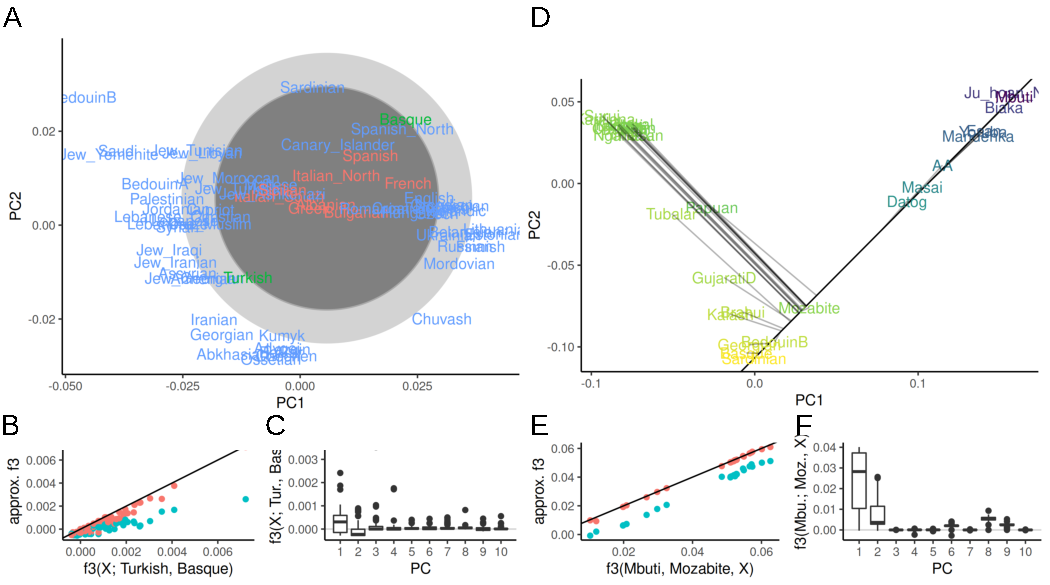
\includegraphics[width=\textwidth]{figures/fig_f3_data.pdf}
	\caption{\textbf{PCA and $F_3$-statistics} A: PCA of Western Eurasian data; the circle denotes the region for which $F_3(X; \text{Basque}, \text{Turkish})$ may be negative. Populations for which $F_3$ is negative are colored in red. B, E: $F_3$ approximated with two (blue) and ten (red) PCs versus the full spectrum. C,F: Contributions of PCs 1-10 to each $F_3$-statistic. D: PCA of World data set, color indicates value of $F_3(\text{Mbuti}; \text{Mozabite}, X)$. The black line shows the projection axis Mbuti-Mozabite, the gray lines indicates the projected position of each population. }
	\label{fig:f3}
\end{figure}

\subsection{$F$-statistics as projections}
The inner product $\langle X_x - X_1, X_x - X_2 \rangle$ is closely related to the projection of a vector onto another one. This interpretation is useful either when calculating an outgroup-$F_3$-statistic, or when we want to find the ``best'' admixture source $X_2$ if we assume the admixed population $X_x$ and one source $X_1$ are known.  The angle between $X_x - X_1$ and $X_x - X_2$ is obtuse if $X_2$ is in the half-plane whose boundary goes through $X_x$ and is orthogonal to $\overline{X_XX_1}$ (Figure \ref{fig:geom}C), and its value is proportional to the projection onto $X_X - X_1$. A common interpretation guide is to use the population which yields the most negative $F_3$-statistic as the population which is most closely related to the ``true'' source of admixture \citep{patterson2012}; on a PCA-plot this corresponds to using the population that is furthest away from $X_x$ on the direction $X_x - X_1$.

This projection argument also helps to interpret Outgroup-$F_3$-statistic on a PCA-plot (Figure \ref{fig:geom}D), but in this case we aim to find the most closely related population as that with the highest $F_3$-statistic. 

\paragraph{Example}
Again, these projection will be orthogonal when using the full data, and may only be approximately orthogonal when approximated using the first two PCs. In Figure \ref{fig:f3}D, I visualize the outgroup-$F_3$-statistic $F_3(\text{Mbuti}; \text{Mozabite}, X_i)$, i.e. a statistic that aims to find the population most closely related to Mozabite (a Berber ethnic group from the northern Sahara), assuming the Mbuti are an outgroup. On a PCA, we can interpret this $F_3$ statistic as the projection of the line segment from $\text{Mbuti}$ to population $X_i$ onto the line through Mbuti and Mozabite (black line). For each population, the projection is indicated with a grey line. In the full data space, this line is always orthogonal to the segment Mbuti-Mozabite, but on the plot (i.e. the subspace spanned by the first two PCs), this is not necessarily the case. We see that particularly the samples from East Asia, Siberia and the Americas project very close to orthogonally, suggesting that most of the variation is captured by these first two PCs, and the coloring based on the full $F_3$-statistics shows that in this case, the first two PCs approximate the $F_3$-statistic very well. We can quantify this and find that the first two PCs slightly underestimate the absolute value of $F_3$ (Figure \ref{fig:f3}E), but keep the relative ordering. This $F_3$-statistic is also very sparse, with e.g. PCs 3-5, 7 and 10 having almost zero contribution to all statistics (Figure \ref{fig:f3}F), and PCs 6, 8 and 9 having a similar non-zero contribution for almost all statistics, likely because these PCs explain within-African variation.


\subsection{$F_4$-statistics as angles}
The interpretation of $F_4$ in PCA is similar to that of $F_3$ as a projection of one vector onto another, with the difference that now all four points may be distinct. As for $F_3$, a finding of $F_4(X_1, X_2; X_3, X_4) = 0$ implies that the vectors $X_1 - X_2$ and $X_3 - X_4$ are orthogonal, or that the two populations map to the same point, and otherwise it will correspond to the length of the projection (Figure \ref{fig:geom}E). 

We can also see how this interpretation aligns with that of $F_4$ as the length of an internal branch on a tree : By assumption, disjoint sets of branches evolve independently \citep{cavalli-sforza1964, felsenstein1973, semple2003}. Since the data space is sufficiently high-dimensional, this ensures that the resulting drift trajectories will also be uncorrelated. Therefore, if we interpret $F_4(X_1, X_2; X_3, X_4)$ as the projection of $X_3 - X_4$ - onto $X_1 - X_2$, we can write  
$$X_3 - X_4  = (X_3 - X'_3) + (X'_3 - X'_4) + (X'_4 - X_4)\text{.}$$ Of these three branches, the first and last are orthogonal to $X_1 - X_2$ and thus the $F_4$ statistic is just the internal branch of the tree (Figure \ref{fig:geom}F). It also suggests a number of diagnostic $F$-statistics that check assumptions; for example if the tree holds, then 
$F_4(X_3, X_3'; X_4, X_4') = 0 $.

Since $F_4$ is a covariance, its magnitude lacks an interpretation. Therefore, commonly correlation coefficients are used, as there, zero means independence and one means maximum correlation. For $F_4$, we can write 
\begin{equation}
\text{Cor}(X_1 - X_2, X_3 - X_4) =  \frac{\langle X_1 - X_2, X_3 - X_4 \rangle}{\norm{X_1-X_2}\norm{X_3-X_3}} = \cos(\phi),\label{eq:angle}
\end{equation}
where $\phi$ is the angle between $X_1 - X_2$ and $X_3 - X_4$. Thus, independent drift events lead to $\cos(\phi) = 0$, so that the angle is 90 degrees, whereas an angle close to zero means $\cos(\phi)\approx 1$, which means most of the genetic drift on this branch is shared.

\paragraph{Example}
To illustrate the angle interpretation I again use the Westeurasian data. The PCA-biplot shows two roughly parallel clines (Figure \ref{fig:f3}A), a European gradient (from Sardinian to Chuvash), and a Asian cline (from Arab to Caucasus populations). This is quantified in Figure \ref{fig:f4}A, where I plot the angle corresponding to $F_4(X, \text{Sardinian}; \text{Saudi}, \text{Georgian})$. For most European populations, using two PCs (green points) gives an angle close to zero, corresponding to a correlation coefficient between the two clines of $r>0.9$. Just adding PC3 (blue), however, shows that the parallelism of the clines is spurious: Using three PCs or the full data (red) shows that most correlations are low. I arrive at a similar interpretation from the spectrum of these statistics (Figure \ref{fig:f4}B), which has high loadings for the first three PCs, with minimal contributions from the higher ones.

\subsection{Other projections}
So far, I used eq. \ref{eq:fpc} to interpret $F$-statistics on a PC-plot, but the argument holds for \emph{any} orthonormal transformation. This allows for a variety of visualizations that use both $F$-statistics and PCs. The motivation for this is that sometimes we wish to partition the variation in the data into a subspace of interest, and an orthogonal residual space that captures the information discarded. Examples where analyses are restricted to such subspaces include the $F_4$-ratio test \citep{patterson2012, petr2019}, \texttt{qpWave} \citep{skoglund2015} and \texttt{qpAdm} \citep{harney2021}. For the $F_4$-ratio, for example, a ratio
\begin{eqnarray}
\alpha = \frac{F_4(R_1, R_2; X, A)}{F_4(R_1, R_2; B, A)}  \label{eq:f4ratio}
\end{eqnarray}
is used, which can be interpreted as projecting $X-A$ and $B-A$ onto $R_1 - R_2$. Thus, we can make a plot where we plot the variation on the $X$-axis along $R_1 - R_2$, and perform a PCA on the residual. This can be important because the residual can be used to check assumptions, e.g. $A - A'$ and $B - B'$ need to be orthogonal (Figure \ref{fig:geom}F).

\subsubsection{Example}
In the PCA on the world overview data set, I found a seemingly linear gradient from Africans to Europeans (Figure \ref{fig:f3}D). I focus on this cline using an alternative projection by using  $F$-statistics of the form $F_4(X, Y; \text{Sardinian}, \text{Yoruba})$), which might e.g. be used if we were to quantify gene flow associated with the out-of-Africa expansion. These $F_4$-statistics are very well-approximated by the first two PCs, with a 99.2\% correlation between $F_4$ and its approximation using the first two PCs (Figure \ref{fig:f4}C).

In Figure \ref{fig:f4}D, I show the projection $\langle X; \text{Sardinian}, \text{Yoruba} \rangle$ on the $X$-axis, which means that $F_4(X, Y; \text{Sardinian}, \text{Yoruba})$ is  is proportional to their horizontal distance between $X$ and $Y$. 
The first two residual PCs are given on the Y-axis and in the coloring; this visualization reveals some variation within Africans (with Mbuti, Biaka and Ju$\vert$'hoansi) that is largely orthogonal to this gradient, as is the variation between Europeans, Asian and the Americans. 

The percentage of between-population variance explained by the Sardinia-Yoruba axis (24\%) is much lower than that of the first PC (40\%, Figure \ref{fig:f4}E). However, the cumulative variance explained by the first two axes is similar, with (52\%) explained when adding residual PC1 to the projection, compared to 55\% for the first two PCs. The advantage of specifying one axis is that it displays the orthogonal components more explicitly, reveals distinct structure in Africans and non-Africans and thus can be used to test assumptions of more complex models.

\begin{figure}[!ht]
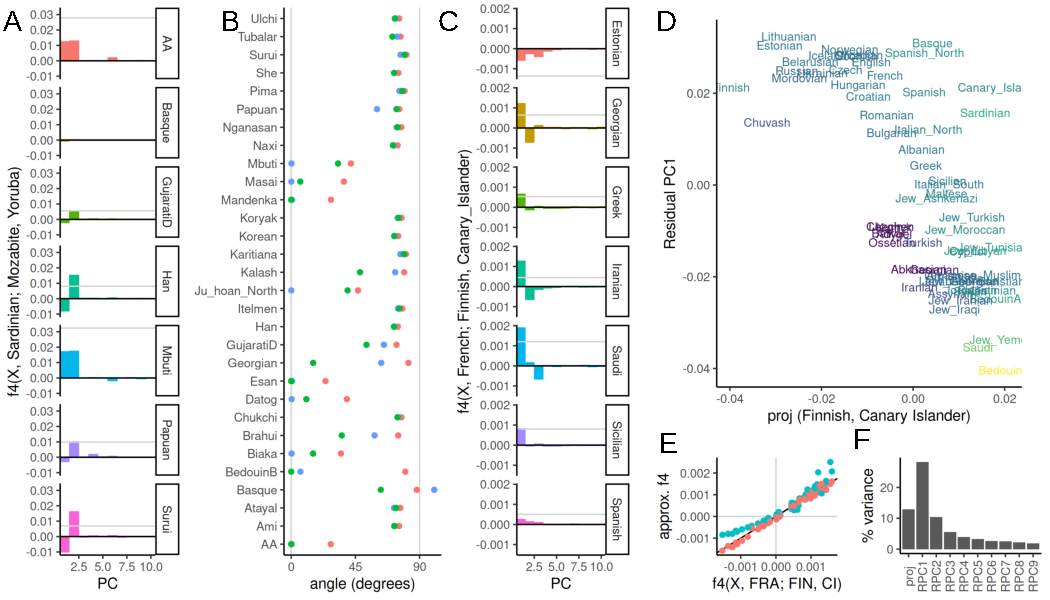
\includegraphics[width=\textwidth]{figures/fig_f4_data.pdf}	
	\caption{\textbf{PCA and $F_4$-statistics} A: Projection angle and correlation coefficient $r$ representation of $F_4(X, Sardinian; Saudi, Georgian)$ (red) in the Westeurasian data set, and approximations using two (green) and three (blue) PCs.
	B: Spectrum of select $F_4$-statistics in the Western Eurasian data set.  C: Spectrum of $F-4$-statistics in World data set. D: Scatterplot of $F_3$-projection on Sardinian-Yoruba axis  and residual PC1.
	E: Percent variance explained from of the projection based on $F_3$ in panel D and first nine residual PCs (light gray), compared with percent variance explained by first ten PCs (dark gray).
	}
\label{fig:f4}
\end{figure}

\section{Discussion}
Particularly for the analysis of ancient DNA, $F$-statistics  are  a powerful tool to describe population genetic diversity. Here, I show that the geometry of $F$-statistics \citep{oteo-garcia2021} leads to a number of simple interpretations of $F$-statistics on a PCA plot. This allows for direct and quantitative comparisons between $F$-statistic-based results and PCA biplots. As PCA is often ran in an early step in data analysis, this also aids in generation of hypotheses that can be more directly evaluated using generative models, (e.g using a lower number of populations). It also allows reconciling apparent contradictions between $F$-statistics and PCA-plots; differences between the two data summaries are explained solely by higher PCs, and so whenever such contradictions arise, and so higher PCs will be informative for population structure. Previous interpretation of PCA in the context of population genetic models have primarily focused on the PCs, which can be derived analytically for trees \citep{cavalli-sforza1975} and homogeneous spatial models \citep{novembre2008a}. My interpretation here is different in that it puts more emphasis on the geometry itself, rather than directly interpreting the PCs. One consequence is that the results here are not impacted by sample ascertainment and sample sizes \citep{mcvean2009, novembre2008a}, which are common concerns in the interpretation of PCA. However, a very skewed sampling distribution will increases the likelihood that more or different PCs will have to be included in the analysis. From this perspective, one could envision a framework where $F$-statistics are used to decide which samples should be included to obtain a low-dimensional PCA-plot ``representative'' of the data

As $F$-statistics are motivated by trees, they assume that populations are discrete, related as a graph, and that gene flow between populations is rare \citep{patterson2012,harney2021}. However, in many regions, all humans populations are admixed to some degree \citep{pickrell2014}, and in regions such as Europe, genetic diversity is distributed continuously \citep{novembre2008, novembre2008a}. This provides a challenge for interpretation; as many $F_3$ and $F_4$ statistics may indicate gene flow. In my example (Figure \ref{fig:f3}A), most Southern European populations are ``admixed'' between Basques and Turkish, but a more accurate model might be one of continuous variation where Basque and Turkish lie on one of multiple gradients; which is more directly visualized with PCA. There are a number of tools that have been developed that use multiple $F$-statistics to build complex models, such as \texttt{qpGraph} \citep{lazaridis2014} and \texttt{qpAdm} \citep{harney2021}. One issue with these approaches is that they are usually restricted to at most a few dozen populations. As ancient DNA data sets now commonly include thousands of individuals, analysts are faced with the challenge of which data to include. A common approach is to sample a large number of distinct models, and retain the ones that are compatible with the data. However, as both \texttt{qpGraph} and \texttt{qpAdm} assume that gene flow is rare and discrete, selecting sets of populations that did experience little gene flow will provide good fits. One example of this is the world foci data set used here, which contains only 33 populations from across the world, and which is well-approximated by two PCs. However, this ascertainment misses a large amount of variation; a more dense sampling would show that in many places human genetic diversity is very gradual and multi-layered \citep{lazaridis2014, peter2020a}. The PCA-based  interpretation offers an alternative that trades interpretability for robustness. Particularly interpreting a (normalized) $F_4$-statistic as a correlation coefficient translates to generalized models of gene flow. Separating $F$-statistics in a sum of model and residuals, and performing a PCA on the latter (such as in Figure \ref{fig:f4}D)  is another way how we can visualize $F$-statistics and evaluate the model fit.

To make this link directly applicable to data analysis, there are a number of -- primarily statistical -- concerns that will need to be addressed. Fist, PCA is most frequently run on individuals, whereas $F$-statistics are often calculated on populations. This is largely because in most workflows, PCA is run much earlier than $F$-statistics; it is a standard assumption of $F$-statistics that there is no population substructure \citep{patterson2012}, and an easy way to test that is ensure that all individuals cluster tightly on a PCA. 

A second difference is that frequently, rare SNPs are weighted higher in PCA, whereas all SNPs are weighted the same for $F$-statistics \citep{patterson2006, patterson2012}. This is a difference of convention \citep{cavalli-sforza1975}; since $F$-statistics are summed over SNPs with the same expectation, $F$-statistics could also be calculated using the same weighting. The close connection between the two approaches developed here suggest that for most analyses, users might want to be consistent and use the same weighting for both types of analyses. 

The third and perhaps biggest gap are statistical issues. The treatment here focuses on the mean estimated $F$-statistic, but many  applications of $F$-statistics are based on hypothesis tests \citep{patterson2012}. This requires estimating accurate standard errors for these statistics, which is difficult since nearby SNPs will be correlated due to recombination \citep{hahn2018}. In contrast, PCA jointly models the covariance matrix due to population structure and sampling, so if hypothesis tests are desired this will need to be incorporated.

An advantage of calculating $F$-statistics based on PCs is that they yield consistent estimtates. For both data sets I investigated here, the matrix $\MF$ of $F$-statistics obtained  using admixtools2 is not a proper squared Euclidean distance matrix, i.e. it is not negative semidefinite and has imaginary PCs. A model-based framework based on probabilistic PCA \citep{hastie2015, meisner2021, agrawal2020} would likely be able to generate consistent $F$-statistics and PCs, while incorporating sampling error and missing data.


\appendix
\section{Derivations}\label{appendix:fonpc}
\setcounter{equation}{0}
\renewcommand{\theequation}{\thesection\arabic{equation}}
Depending on a readers' background in linear algebra, these results may appear elementary; I include them here for reference and because they were not obvious to me at the onset of this project.
\paragraph{$F$-statistics are invariant under a change-of-basis}
\begin{eqnarray}
F_2(X_i, X_j) &=& \sum_{l=1}^L \big( (x_{il} - \mu_l) -(x_{jl} -\mu_l)\big)^2 = F_2(Y_i, Y_j)\nonumber\\
&=& \sum_{l=1}^L \big( \sum_k L_{kl}P_{ik} - \sum_kL_{kl}P_{kj}\big)^2\nonumber\\
&=& \sum_{l=1}^L \left( \sum_k L_{kl} (P_{ik} -P_{jk}) \right)^2\nonumber\\
&=& \sum_{l=1}^L \left( \sum_k L_{kl}^2 (P_{ik} -P_{jk})^2 + 2\sum_{k\neq k'} L_{kl}L_{k'l}(P_{ik} - P_{jk'})^2 \right)\nonumber\\
&=& \sum_k \underbrace{\left(\sum_{l=1}^L L_{kl}^2\right)}_1 (P_{ik} -P_{jk})^2 + 2\sum_{k\neq k'}\underbrace{\left(\sum_{l=1}^L L_{kl}L_{k'l}\right)}_{0} (P_{ik} - P_{jk'})^2\nonumber\\
&=& \sum_k (P_{ik} - P_{jk})^2 \label{eq:changeofbasis}
\end{eqnarray}

In summary, the first row shows that $F_2$ on the centered data will give the same results (as distances are invariant to translations), in the second row we apply the PC-decomposition. The third row is obtained from factoring out $L_{lk}$. Row four is obtained by multiplying out the sum inside the square term for a particular $l$. We have $k$ terms when for $\binom{k}{2}$ terms for different $k$'s.  Row five is obtained by expanding the outer sum and grouping terms by $k$.The final line is obtained by recognizing that $\ML$ is an orthonormal basis; where dot products of different vectors have lengths zero.

Note that if we estimate $F_2$, unbiased estimators are obtained by subtracting the population-heterozygosities $H_i, H_j$ from the statistic. As these are scalars, they do not change above calculation.

\paragraph{The region of negative $F_3$-statistics is a $n$-ball}
Without loss of generality, assume that $X_1 = (r, 0, 0, \dots)$ and $X_2 = (-r, 0, 0, \dots)$, and let us assume that $X_x$ has coordinates $(x_1, x_2, \dots, x_S)$ Assuming $F_3(X_x; X_1, X_2) = 0$, equation \ref{eq:f3neg} becomes
\begin{align}
2 F_3(X_x; X_1, X_2) &=  \normsq{X_x - X_1} + \normsq{X_x - X_2}  - \normsq{X_1 - X_2} = 0 \nonumber\\
&= \left[(x_1-r)^2 + \sum_{i=2}^S x_i^2\right] + \left[(x_1 + r)^2 + \sum_{i=2}^S x_i^2\right] - 4r^2 \nonumber\\
&= 2 \left[\sum_{i=1}^S x_i^2 + r^2 + x_1r - x_1r\right] - 4r^2\nonumber\\
F_3(X_x; X_1, X_2) & = -r^2 + \sum_{i=1}^S x_i^2 = -r^2 + \normsq{X_x} = 0  \text{,} \label{eq:f3sphere}
\end{align}
which is the equation of a $n$-sphere with radius $r$ and center at the origin, as assumed from the placing of $X_1$ and $X_2$. Now, assume that $F_3$ is negative, i.e. $F_3(X_x; X_1, X_2) = -k < 0$. Moving $r^2$ to the left we obtain
\begin{equation}
r^2 - k = \normsq{X_x} \text{,}
\end{equation}
which is another $n$-sphere with a smaller radius, showing that all points inside the $n$-sphere will have negative $F_3$-values.

\paragraph{If a population lies outside the circle of this $n$-Sphere in any 2D-projection, $F_3$ is positive} 
Assume the center of the $n$-sphere $C = \frac{X_1 + X_2}{2} = (c_1, c_2, \dots c_S)$, and $X_x = (x_1, x_2, \dots x_S)$.  Then, 
\begin{align}
F_3(X_x; X_1, X_2) &= \normsq{X_x - C} - r^2 \nonumber\\
&= \underbrace{(x_1 - c_1)^2 + (x_2 - c_2)^2}_{>r^2} + \underbrace{\sum_{i=3}^S (x_i - c_i)^2}_{\geq 0} - r^2 \nonumber\\
& > 0 \text{.}\label{eq:f3circle}
\end{align}
The condition $(x_1 - c_1)^2 + (x_2 - c_2)^2 >r^2$ is satisfied whenever $X_x$ is outside the circle obtained from projecting the $n$-sphere on the first two dimensions. An analogous argument applies for any low-dimensional representation.

\bibliographystyle{plainnat}
\bibliography{main}

\end{document}
